\documentclass[]{article}

% to define bibliography and insert cites
\usepackage[backend=biber]{biblatex}
\addbibresource{references.bib}

% multilanguage
\usepackage[english,spanish]{babel} 

\newenvironment{poliabstract}[1]
	{\renewcommand{\abstractname}{#1}\begin{abstract}}
	{\end{abstract}}

% to insert fragments of code
\usepackage{listings}

% to make links clickable
\usepackage{hyperref}
\hypersetup{colorlinks=false,linktoc=all}

% include images
\usepackage{graphicx}
\usepackage{caption}    % contains subpackage 'subcaption'
\usepackage{subcaption} % allows subfigures
\usepackage{float}      % allows floating H to place images in certain place

% paragraph spacing
\usepackage{parskip}
\usepackage{setspace}

% avoid numbering in equation
\usepackage{amsmath}

% coloring text
\usepackage{xcolor}

% beautiful tables
\usepackage{booktabs}

% caption font
\usepackage{caption}
\captionsetup[figure]{font=small, labelfont=bf}
\captionsetup[table]{font=small, labelfont=bf}

% language redefinitions
\addto\captionsspanish{%
	\renewcommand*\contentsname{Contenido}
	\renewcommand{\figurename}{Figura}
	\renewcommand{\tablename}{Tabla}
}

\begin{document}

\begin{titlepage}
	\centering
	\includegraphics[width=0.5\textwidth]{images/logo_utad.jpg}\par\vspace{1cm}
	{\large\bfseries Sistema de detección automática de baches en el asfalto a partir de imágenes\par}
	\vspace{1.5cm}
	{\large \itshape Diego Castro Viadero\par}
	Septiembre 2019\par
	\vspace{1.5cm}
	{\small Tutor: Ricardo Moya García}
\end{titlepage}

\selectlanguage{spanish}
\begin{abstract}
El estado del asfalto en carreteras tanto de ámbito nacional como de ámbito urbano es de alta importancia en relación a la seguridad vial. En la actualidad, no existe un sistema de detección automática de socavones en el asfalto. Tan sólo se tiene conocimineto de los mismos cuando han sido los causantes de un accidente vial o de una queja ciudadana (detección pasiva).

Este proyecto pretende desarrollar un sistema de detección automática y activa de socavones a partir de imágenes, que permita a las autoridades pertinentes conocer el número y ubicación de los mismos. Los principales objetivos son:

\begin{itemize}
	\item Detección temprana y activa de socavones a partir de imágenes
	\item Creación de una base de datos con la relación de socavones detectados (número y ubicación)
\end{itemize}

Los principales beneficios son:

\begin{itemize}
	\item Optimización de recursos necesarios para la reparación de socavones
	\item Aumentar la seguridad vial de las carreteras y evitar accidentes
	\item Aumentar la satisfacción de la ciudadanía en relación al estado de las carreteras de su municipio
\end{itemize}
\end{abstract}

\selectlanguage{english}
\begin{abstract}
{\color{red} \textbf{!!! TODO}}
\end{abstract}

\newpage
\selectlanguage{spanish}
\tableofcontents{}

\newpage
\section{Introducción}

\subsection{Motivación}

En los últimos años las prioridades en relación a la seguridad vial han provocado un cambio de mentalidad en la sociedad.  Muchos de los últimos avances tecnológicos están orientados al desarrollo de medios de transporte más seguros. Uno de estos avances que contribuye a la mejora de la seguridad es la inclusión de un sistema de detección de desperfectos en la calzada.

En la actualidad, en el ayuntamiento de Madrid, existe un sistema de sugerencias y reclamaciones \cite{s1_syr} que permite al ciudadano, entre otras opciones, denunciar la existencia de irregularidades en el asfalto, tener un registro de las mismas y planificar su subsanación. Según el informe de sugerencias y reclamaciones del ayuntamiento de Madrid \cite{s1_syrreport}, en el primer semestre del año, se registraron 3.000 reclamaciones en materia de \textit{vías y espacios públicos} de las cuales el 50\% correspondieron a la submateria \textit{aceras y calzadas}.

Este sistema de funcionamiento actual, que delega en el ciudadano la tarea de reporte de este tipo de desperfectos, dificulta y retrasa la puesta en conocimiento de las irregularidades a las autoridades responsables aumentando la probabilidad de que suceda algún incidente.

Algunas marcas de vehículos han desarrollado innovaciones, que son capaces de detectar baches cuando pasan sobre ellos y adaptar la dureza de la suspensión para conseguir una conducción más segura y cómoda. También contemplan un envío sistemático de la detección de baches, en tiempo real, tanto a otros vehículos como a las autoridades pertinentes. Otras marcas plantean la inclusión de cámaras que permitan la detección del bache sin necesidad de pasar por encima de este.

Con estas innovaciones se recupera el control sobre la detección de baches, liberando al ciudadano de esta tarea y reduciendo la probabilidad de incidentes gracias a disponer de la información con más antelación.

\subsection{Objetivos}

Este trabajo trata de desarrollar un sistema de detección de baches en tiempo real en línea con los últimos avances tecnológicos. El objetivo es entrenar una red neuronal con un conjunto de imágenes donde los baches han sido etiquetados previamente y obtener como resultado un modelo exportable para ser ejecutado en un dispositivo móvil.

Gracias a este trabajo he podido ampliar los conocimientos adquiridos durante el máster de Big Data \& Data Science, impartido por la U-TAD, centrando el proyecto en el procesamiento de imágenes y tratando al mimso tiempo que tenga una utilidad social.

\subsection{Estructura del trabajo}

La sección \textit{\nameref{sec:estado_del_arte}} explica cómo se pueden solucionar este tipo de problemas, y se centra en la resolución de los mismos mediante el uso de redes neuronales, valorando los pros y contras de cada uno de ellas.

La sección \textit{\nameref{sec:definicion_de_requisitos_y_analisis}} realiza un análisis de requisitos del proyecto y plantea una arquitectura para su desarrollo.

La sección \textit{\nameref{sec:datos}} describe el conjunto de datos utilizado, el análisis exploratorio que se ha realizado sobre el mismo y el preprocesamiento que se realiza sobre los datos antes de ser utilizados.

La sección \textit{\nameref{sec:tecnicas_de_deep_learning_y_metodos_de_evaluacion}} realiza una descripción a nivel teórico de las principales técnicas y conceptos que se aplican en el tipo de red neuronal seleccionada para el desarrollo del proyecto. También describe las métricas que se utilizan para evaluar los modelos generados.

La sección \textit{\nameref{sec:implementacion_y_evaluacion_de_las_tecnicas}} describe cómo se ha implementado la red neuronal y el resultado de la evaluación de los modelos generados.

La sección \textit{\nameref{sec:resultados}} muestra algunos ejemplos concretos obtenidos con los distintos modelos generados.

La sección \textit{\nameref{sec:conclusiones}} contiene una valoración del proyecto y se comentan posibles mejoras a realizar. % (2-4 páginas)

\newpage
\section{Estado del arte}

% En el punto de motivación y objetivos debes de dejar muy claro que es lo que quieres hacer (un detector de baches) y en este tema 2 debes de explicar como se solucionan este tipo de problemas (CNN) y las redes y frameworks existentes para poder realizar tu trabajo. Como esto ya es una cosa que has hecho (me lo mandaste en un mail muy bien explicado) debes de contar los pros y contras y justificar el porque has seleccionado la red seleccionada

Con respecto al cómo afrontar el problema, he visto que existen 2 maneras de hacerlo:

- clasificación de imágenes
- identificación de objetos

El primero de los enfoques es más sencillo y está más estudiado. Dada una imagen centrada en un objeto, determinar de qué clase es el objeto. La forma de resolverlo sería con una red neuronal convolucional. Ya existen distintas arquitecturas de redes convolucionales estudiadas para resolver este tipo de problemas (VGG-16, LeNet, ResNet, GoogLeNet/Inception, etc.). Dudo de si este sería un enfoque válido para el problema en cuestión ya que las imágenes no están centradas en los baches y los baches representan una superficie ínfima de la imagen.

El segundo de los enfoques es más complicado y está en continua mejora en los últimos años.

Existen dos formas para resolver este problema:

- técnicas de machine learning clásicas (Viola-Jones [HAR], HOG + SVM)
- deep learning

El uso del deep learning es lo que ha supuesto una revolución y es el que está en continua mejora en los últimos años. Las principales técnicas usando Deep learning son:

- R-CNN
- Fast R-CNN
- Faster R-CNN
- SDD
- YOLO (YOLO, YOLOv2, YOLOv3)
- Mask R-CNN % (como mucho 10 páginas)

\newpage
\section{Definición de requisitos y análisis}
\label{sec:definicion_de_requisitos_y_analisis}

\subsection{Definición de requisitos}

% (que se quiere hacer definido de una manera formal)
% descripción del caso de uso

{\color{red} \textbf{!!! TODO}}

\subsection{Arquitectura}

% (Haz un diagrama y luego explicalo, asi te valdrá para la presentación del proyecto)
% diagrama sencillo con la arquitectura: fotos + red neuronal + modelo + móvil

\begin{figure}[H]
	\centering
	\includegraphics[width=\linewidth]{images/architecture.png}
	\caption{Arquitectura de la solución}
	\label{fig:architecture}
\end{figure}

{\color{red} \textbf{!!! TODO}}

\subsection{Tecnologías}

% (Esto es poco más que enumerar lo que vas a utilizar)
% python, keras, tensorflow, opencv, java, yolo v3, yolo v3 tiny

{\color{red} \textbf{!!! TODO}} % (2-4 páginas)

\newpage
\section{Datos}
\label{sec:datos}

\subsection{Descripción de las fuentes de datos a utilizar}

El juego de datos, utilizado para realizar el entrenamiento de la red YOLO, ha sido obtenido de kaggle \footnote{https://www.kaggle.com/felipemuller5/nienaber-potholes-2-complex}. Está compuesto por un total de 1900 imágenes, tomadas desde el interior de un coche, con una resolución de 3680x2760 píxeles (formato 4:3). El juego de datos también consta de un conjunto de ficheros de texto con el etiquetado de las imágenes. Las imágenes se organizan en dos subconjuntos: uno de 1297 imágenes para el entrenamiento y otro de 603 imágenes para la evaluación del modelo. Por cada uno de los subconjuntos de imágenes existe un fichero de texto con el etiquetado de las mismas. Cada una de las líneas del los ficheros de texto contiene las etiquetas de una imagen. La estructura de cada línea es la siguiente:

\begin{lstlisting}[frame=single,basicstyle=\ttfamily\footnotesize]
<RUTA_IMG> <NUMERO_DE_ETIQUETAS>( <X0> <Y0> <ANCHO> <ALTO>)+
\end{lstlisting}

\subsection{Estudio de los datos}

El primer paso que se ha realizado es hacer un estudio de los datos, concretamente se ha hecho un análisis del tamaño de los baches con respecto al tamaño de la imagen. Este es un aspecto importante a tener en cuenta, ya que los algoritmos de detección de objetos son sensibles a este factor y por lo general se comportan peor cuanto más pequeños son los objetos a detectar. Precisamente una de las mejoras que se han conseguido en la última versión de YOLO es la detección de objetos pequeños.

Como se puede observar en la figura \ref{fig:potholesizes}, la mayoría de los baches tienen una anchura inferior a 200 píxeles y una altura inferior a 50 píxeles. Este es un tamaño muy pequeño con respecto a la imagen (3680x2760) y hará difícil su detección.

\begin{figure}[H]
	\centering
	\includegraphics[width=0.7\linewidth]{images/pothole_sizes_scatter_plot.png}
	\caption{Tamaños de los baches en píxeles}
	\label{fig:potholesizes}
\end{figure}

También se ha realizado un estudio de la localización de los baches en las imágenes. Tal y como se ve en la figura \ref{fig:potholeslocations}, los baches están localizados principalmente en el centro de la imagen. La parte inferior se corresponde con el salpicadero del coche y la parte superior se corresponde con paisaje.

\begin{figure}[H]
	\centering
	\includegraphics[width=0.7\linewidth]{images/pothole_locations_heatmap.png}
	\caption{Localizaciones de los baches en las imágenes}
	\label{fig:potholeslocations}
\end{figure}

\subsection{Preparación de las imágenes}
\label{subsec:preprocesamiento_de_las_imagenes}

Tanto en la fase de entrenamiento, como para hacer una predicción, las imágenes van a ser redimensionadas al tamaño de la red neuronal, la cual tiene una relación de aspecto 1:1, sin embargo las imágenes del juego de datos tienen una relación de aspecto 4:3.

Para redimensionar una imagen con una relación de aspecto 4:3, y al mismo tiempo, transformarla en una imagen con relación de aspecto 1:1, lo que se hace es redimensionar el lado más grande de la imagen manteniendo la relación de aspecto, es decir, se aplica el mismo factor de redimensionamiento al lado más pequeño. Una vez redimensionada, se rellena con gris la zona superior y la zona inferior de la imagen para cuadrarla. En la figura \ref{fig:imagedirectresize} se muestra un ejemplo gráfico.

\begin{figure}[H]
	\centering
	\begin{subfigure}[h]{0.45\linewidth}
		\includegraphics[width=\linewidth]{images/image_direct_resize_before.jpg}
	\end{subfigure}
	\begin{subfigure}[h]{0.45\linewidth}
		\includegraphics[width=\linewidth]{images/image_direct_resize_after.jpg}
	\end{subfigure}
	\caption{A la izquierda la imagen original redimensionada a tamaño 920x690 px (manteniendo la relación de aspecto 4:3). A la derecha la imagen redimensionada con el relleno para que tenga una relación de aspecto 1:1 (920x920 px)}
	\label{fig:imagedirectresize}
\end{figure}

El redimensionamiento se hace en base al lado más grande de la imagen, que en el ejemplo anterior es la anchura. Para calcular el factor de redimensionamiento, se divide la anchura de la imagen final entre la anchura de la imagen original. En este caso, como se quiere redimensionar la imagen a una anchura de 920 píxeles, el factor de redimensionamiento es: $920 / 3680 = 0.25$. A continuación, se aplica este factor de redimensionamiento a ambos lados de la imagen, resultando en un tamaño de 920x690 píxeles. Por último se calcula el relleno que hace falta a cada lado de la imagen: $(920 - 690) / 2 = 115$.

Siguiendo con este ejemplo, si en la imagen original hubiese un bache de tamaño 160x24 píxeles, y se aplicase este factor de redimensionamiento ($0.25$), el bache redimensionado tendría unas dimensiones de 40x6 píxeles, lo cual sería un tamaño bastante pequeño ya que únicamente tiene 6 píxeles de alto (de los 920 que tiene la imagen).

Sin embargo, si previo al redimensionamiento de la imagen, se recortan los extremos izquierdo y derecho de la imagen, de tal forma que tenga una relación de aspecto 1:1, se consigue que el factor de redimensionamiento sea mayor y que por tanto los baches redimensionados sean también más grandes. Esta técnica tiene un inconveniente, y es que la imagen original se está recortando, por lo que está habiendo una pérdida de información. Este inconveniente no es un impedimento, ya que en el apartado ~\ref{subsec:preprocesamiento_de_las_imagenes} se ha comprobado que la mayor parte de los baches están en el centro de las imágenes, y que recortando los extremos de las mismas la pérdida de información es mínima.

Para aplicar esta técnica, en primer lugar habría que calcular los recortes que hay que hacer a cada lado de la imagen original. Para ello se calcula la diferencia entre la anchura y la altura de la imagen y se divide por dos: $(3680 - 2760) / 2 = 460$. Tras recortar 460 píxeles a cada lado de la imagen se obtiene una imagen de 2760x2760 píxeles. A continuación se calcula el factor de redimensionamiento: $920 / 2760 = 0.333$. Por último se aplica este factor de redimensionamiento a la altura y la anchura de la imagen.

Si aplicásemos este nuevo factor de redimensionamiento al hipotético bache del ejemplo anterior (de tamaño 160x24 píxeles), el tamaño del bache redimensionado sería 53x8, resultando un 75\% más grande.

Todas las imágenes del juego de datos han sido recortadas de esta forma para que al ser redimensionadas, cuando vayan a ser procesadas por el modelo, los baches sean lo más grandes posibles. % (<4 páginas)

\newpage
\section{Técnicas de Deep Learning y métodos de evaluación}
\label{sec:tecnicas_de_deep_learning_y_metodos_de_evaluacion}

\subsection{Técnicas de Deep Learning a utilizar en el proyecto}

A continuación se explicarán las principales técnicas utilizadas para el desarrollo del proyecto. Algunas de las técnicas que se mencionan no son específicas del deep learning.

\subsubsection*{\textit{Hold-out}}

El entrenamiento de las redes neuronales YOLO se ha realizado siguiendo esta técnica. Hold-out no es una técnica específica del deep learning, sino que es una técnica general que aplica sobre cualquier algoritmo de aprendizaje. Consiste en dividir el conjunto de datos en dos subconjuntos: uno que se utiliza para el entrenamiento y otro que únicamente se utiliza para evaluar el modelo obtenido tras el entrenamiento.

\subsubsection*{\textit{Red Neuronal Convolucional (CNN)}}

Tal y como se ha comentado en el apartado \textit{\nameref{sec:estado_del_arte}}, YOLO es una red neuronal convolucional, por lo que antes de entrar en los detalles se va a explicar cómo funciona una CNN \cite{s5_cnn1} \cite{s5_cnn2} \cite{s5_cnn3}.

Las CNNs están compuestas por una sucesión de capas convolucionales, para la extracción de características, seguidas de unas capas perceptrón simples, para la clasificación final. Las capas convolucionales forman una jerarquía, de forma que las capas del principio son capaces de detectar formas básicas y cuanto más ``profunda'' es la capa, más complejas son las formas que son capaces de detectar. Por ejemplo: una capa inicial sería capaz de detectar líneas y círculos, mientras que una capa profunda sería capaz de detectar una cara.

Cada capa convolucional recibe como entrada una matriz bidimensional. En el caso de tratarse de la primera capa la entrada se corresponde directamente con la imagen, si se trata de una capa más profunda la entrada se corresponde con la salida de la capa anterior. Además, cada capa tiene definido un \textit{kernel}, que no es más que otra matriz bidimensional de dimensiones reducidas. Con la matriz de entrada y el kernel se realiza la operación de \textit{convolución}.

\begin{figure}[H]
	\centering
	\includegraphics[width=0.7\linewidth]{images/convolutional_neuron_example.png}
	\caption{Ejemplo de capa convolucional con una entrada de 5x5 y un kernel de 3x3}
	\label{fig:cnn_neuronex}
\end{figure}

La operación de \textit{convolución} consiste en hacer un barrido del \textit{kernel} por la matriz de entrada, de izquierda a derecha y de arriba a abajo. En cada una de las posiciones del barrido se aplica el producto escalar entre el kernel y la submatriz de la matriz de entrada sobre la que se encuentre. En la figura \ref{fig:cnn_convolutionoperationex} se puede ver gráficamente el proceso.

\begin{figure}[H]
	\centering
	\includegraphics[width=0.7\linewidth]{images/convolutional_operation_example.png}
	\caption{Representación gráfica de operación convolucional}
	\label{fig:cnn_convolutionoperationex}
\end{figure}

Para realizar el producto escalar, las matrices se \textit{aplanan}, de tal forma que la submatriz de entrada quedaría de la siguiente forma:

\begin{equation}
	\left[
	\begin{array}{ccc}
		0 & 1 & 1 \\
		0 & 1 & 1 \\
		0 & 1 & 1 \\
	\end{array}
	\right]
	=>
	\left[
	\begin{array}{ccccccccc}
		0 & 1 & 1 & 0 & 1 & 1 & 0 & 1 & 1 \\
	\end{array}
	\right]
	\nonumber
\end{equation}

El kernel:

\begin{equation}
	\left[
	\begin{array}{ccc}
		0 & 1 & 0 \\
		0 & 1 & 0 \\
		0 & 1 & 0 \\
	\end{array}
	\right]
	=>
	\left[
	\begin{array}{ccccccccc}
		0 & 1 & 0 & 0 & 1 & 0 & 0 & 1 & 0 \\
	\end{array}
	\right]
	\nonumber
\end{equation}

Y por lo tanto el producto escalar:

\begin{equation}
	\left[
	\begin{array}{ccccccccc}
		0 & 1 & 1 & 0 & 1 & 1 & 0 & 1 & 1 \\
	\end{array}
	\right]
	\left[
	\begin{array}{c}
		0 \\
		1 \\
		0 \\
		0 \\
		1 \\
		0 \\
		0 \\
		1 \\
		0 \\
	\end{array}
	\right] = 3
	\nonumber
\end{equation}

Como resultado de aplicar la convolución sobre la matriz de entrada se obtiene una nueva matriz. Además del kernel, las capas convolucionales tienen otros parámetros asociados, como por ejemplo, cómo de rápido avanza el kernel durante el barrido.

Las capas convolucionales no tiene un único kernel asociado, sino que tienen varios. Teniendo en cuenta esto y suponiendo que tenemos como entrada una imagen en blanco y negro de $28x28x1$ píxeles y que cada capa tiene $32$ kernels de $3x3$, la primera capa convolucional estaría compuesta por $28 x 28 = 784$ neuronas, y tras aplicar la operación de convolución, se obtendrían como resultado $32$ nuevas matrices de dimensiones $26 x 26$, que harían necesarias $26 x 26 x 32 = 21.632$ neuronas en la segunda capa. Teniendo en cuenta que una CNN puede estar compuesta por varias decenas de capas, se hace necesario introducir un mecanismo de reducción, para que el número de neuronas necesarias no crezca tan desmesuradamente con cada capa. Este mecanismo se conoce como \textit{pooling}. El \textit{MaxPooling}, es un tipo de pooling comunmente usado, y consiste en deslizar una ventana bidimensional sobre la matriz de entrada, de izquierda a derecha y de arriba a abajo. En cada una de las posiciones se tomará como valor resultante el máximo valor presente en la ventana. La capacidad de reducción del MaxPooling depende de dos factores: el tamaño de la ventana y el tamaño del salto que se da hacia la derecha y hacia abajo. En la figura \ref{fig:cnn_maxpooling} se muestra un ejemplo gráfico.

\begin{figure}[H]
	\centering
	\includegraphics[width=0.7\linewidth]{images/maxpooling_example.png}
	\caption{Representación gráfica de MaxPooling con una entrada de 4x4, una ventana de 2x2 y un salto de 2}
	\label{fig:cnn_maxpooling}
\end{figure}

\subsubsection*{Transferencia de conocimiento (transfer learning)}

% Otra de las técnicas que se han utilizado en el proyecto es la denominada \textit{transferencia del conocimiento (transfer learning)} \cite{s5_transfer_learning}.

Entrenar un modelo de detección de objetos es un proceso muy costoso, ya que se necesita un gran volumen de imágenes y una gran capacidad de cómputo. El \textit{transfer learning} \cite{s5_transfer_learning} viene a paliar este problema ya que permite utilizar un modelo ya entrenado como punto de partida para entrenar otro. Como se ha comentado anteriormente, las primeras capas de una CNN son capaces de detectar formas básicas y a medida que se profundiza en las capas, estas detectan formas más específicas. Si ya tenemos entrenado un modelo \texttt{X} para detectar un determinado tipo de objetos y queremos entrenar otro \texttt{Y} para detectar otro tipo de objetos, las primeras capas de ambos modelos van a detectar el mismo tipo de formas, y serán las capas más profundas las que se diferencien. Por lo tanto podríamos utilizar el modelo \texttt{X} como punto de partida para el modelo \texttt{Y}, y este último podrá beneficiarse del conocimiento transferido aprender más rápido.

Esta técnica se ha utilizado ampliamente durante la fase de entrenamiento. Se ha utilizado para aprovechar el conocimiento de los modelos YOLO ya entrenados proporcionados por sus autores. También se ha utilizado para lidiar con las limitaciones de uso que tiene la infraestructura utilizada durante el entrenamiento.

\subsubsection*{YOLO V3}

En la figura \ref{fig:yolov3architecture} se muestra la arquitectura de YOLO V3 de tamaño 416x416. Está compuesta por un total de 106 capas convolucionales. Tiene una única entrada, de dimensiones 416x416x3, y tres salidas de dimensiones 13x13x255, 26x26x255 y 52x52x255 respectivamente. Las tres salidas se corresponden con 3 escalas de detección de objetos, la primera de ellas sirve para detectar objetos grandes, la segunda objetos medianos y la tercera objetos pequeños.

Como se explicó en la sección \textit{\nameref{sec:estado_del_arte}}, YOLO divide la imagen en una rejilla de $SxS$ celdas. En realidad, divide la imagen en tres rejillas que se corresponden con las 3 salidas. Para cada una de las celdas de estas rejillas se proponen un número $B$ regiones candidatas, en este caso son 5. Cada una de estas regiones candidatas están representadas por 5 variables, 4 para la región propiamente dicha y 1 para indicar la probabilidad de que la región contenga un objeto. YOLO es capaz de detectar 80 clases de objetos, por lo que junto a cada región candidata se añaden otras 80 variables para indicar la probabilidad de pertenencia a cada una de las clases. Con todo esto, cada una de las celdas de las rejillas se compone de $3 x (5 + 80) = 255$ variables.

\begin{figure}[H]
	\centering
	\includegraphics[width=\linewidth]{images/yolo_v3_architecture.png}
	\caption{Arquitectura de YOLO V3 de tamaño 416x416}
	\label{fig:yolov3architecture}
\end{figure}

\subsubsection*{YOLO V3 Tiny}

En la figura \ref{fig:yolov3tinyarchitecture} se muestra la arquitectura YOLO V3 Tiny de tamaño 416x416. Está compuesta por un total de 13 capas convolucionales. Tiene una única entrada, de dimensiones 416x416, y dos salidas de dimensiones 13x13x255 y 26x26x255 respectivamente. El fundamento es el mismo que en YOLO V3. Se han reducido el número de capas convolucionales de manera considerable, lo cual simplifica el modelo y hace que sea apto para ejecutarse en un dispositivo con recursos limitados manteniendo la premisa de ser capaz de detectar objetos en tiempo real.

\begin{figure}[H]
	\centering
	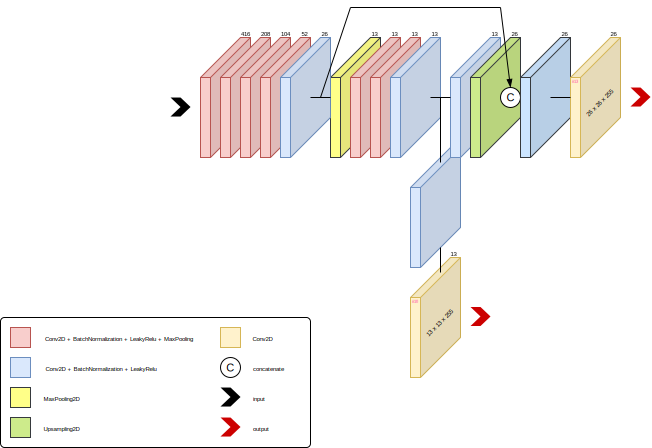
\includegraphics[width=\linewidth]{images/yolo_v3_tiny_architecture.png}
	\caption{Arquitectura de YOLO V3 Tiny de tamaño 416x416}
	\label{fig:yolov3tinyarchitecture}
\end{figure}

\subsection{Métodos de evaluación a utilizar en el proyecto}

La métrica que se ha utilizado para evaluar los modelo obtenidos es la \textit{AP} (Average Precision), que es la métrica que se utiliza en los problemas de detección de objetos.

Antes de explicar en qué consiste la métrica \textit{AP} hay que explicar una serie de conceptos en los cuales está basada: IoU (intersección sobre la unión), precisión (precision) y sensibilidad (recall).

El concepto de \textit{IoU} mide cuánto se solapan dos regiones: la predicha y la que debería ser detectada. Se calcula dividiendo la región obtenida mediante la intersección de la región predicha y la región a detectar entre la región obtenida mediante la unión de ambas regiones.

\begin{equation}
	AP = \frac{interseci\acute{o}n}{uni\acute{o}n} = \frac{\includegraphics[width=0.2\linewidth]{images/ap_intersection.png}}{\includegraphics[width=0.2\linewidth]{images/ap_union.png}}
	\nonumber
\end{equation}

La \textit{precisión} (precision) mide la capacidad del modelo para detectar únicamente los objetos relevantes. Se calcula como el porcentaje de predicciones positivas acertadas frente a todas las predicciones positivas predichas:

\begin{equation}
	precisi\acute{o}n = \frac{TP}{TP + FP} = \frac{TP}{todas\ las\ predicciones\ positivas}
	\nonumber
\end{equation}

La \textit{sensibilidad} (recall)  mide la capacidad del modelo para detectar todos los objetos relevantes. Se calcula como el porcentaje de predicciones positivas acertadas frente a todas las existentes:

\begin{equation}
	sensibilidad = \frac{TP}{TP + FN} = \frac{TP}{todas\ las\ regiones\ a\ detectar}
	\nonumber
\end{equation}

Tanto en el cálculo de la \textit{precisión} como en de la \textit{sensibilidad}, para determinar si una predicción es positiva, se utiliza el \textit{IoU}. Se define un umbral para el \textit{IoU} (normalmente suele ser 0.5) y si se supera dicho umbral, la predicción es considerada positiva.

La métrica \textit{AP} se calcula como el área debajo de la curva \textit{precisión-sensibilidad} (precision-recall). En el eje de las abscisas se representa la \textit{sensibilidad} (recall) y en el eje de las ordenadas se representa la \textit{precisión} (precision).

A continuación se va a mostrar un ejemplo práctico de cómo se calcula la \textit{AP}. Para este ejemplo se dispone de una serie de imágenes con un total de 4 baches a detectar. En la tabla \ref{tab:apprecisionrecalltable} se puede ver el cálculo de la \textit{precisión} y de la \textit{sensibilidad} para las predicciones obtenidas. La columna \textit{Positivo} indica si la predicción es positiva, es decir, si el valor de \textit{IoU} supera el umbral definido, que en este caso es 0.5. Las columnas \textit{TP} y \textit{FP} muestran el acumulado de sus respectivos valores.

\begin{table}[H]
	\centering
	\begin{tabular}{rrrrrr}
		\toprule
		IoU &  Positivo &  TP &  FP &  Precisión &  Sensibilidad \\
		\midrule
		0.912933 &         1 &   1 &   0 &   1.000000 &          0.25 \\
		0.711111 &         1 &   2 &   0 &   1.000000 &          0.50 \\
		0.387983 &         0 &   2 &   1 &   0.666667 &          0.50 \\
		0.387983 &         0 &   2 &   2 &   0.500000 &          0.50 \\
		0.387983 &         0 &   2 &   3 &   0.400000 &          0.50 \\
		1.000000 &         1 &   3 &   3 &   0.500000 &          0.75 \\
		0.225986 &         0 &   3 &   4 &   0.428571 &          0.75 \\
		0.225986 &         0 &   3 &   5 &   0.375000 &          0.75 \\
		1.000000 &         1 &   4 &   5 &   0.444444 &          1.00 \\
		\bottomrule
	\end{tabular}
	\caption{Cálculo de la precisión y sensibilidad para las predicciones}
	\label{tab:apprecisionrecalltable}
\end{table}

Una vez se tienen calculados los valores de \textit{precisión} y de \textit{sensibilidad} se calcula la curva \textit{precisión-sensibilidad} como se puede ver en la figura \ref{fig:apprecisionrecallcurve}. Para realizar el cálculo del área debajo de la curva se realiza un suavizado de la misma. Este suavizado consiste en establecer como valor de \textit{precisión} para un determinado valor de \textit{sensibilidad}, el valor de \textit{precisión} más alto que se encuentre a su derecha. Por ejemplo, para la \textit{sensibilidad} 0.6 se establece como valor de \textit{precisión} el valor más alto a su derecha, que en este caso es 0.5. En color naranja se puede ver la curva suavizada.

\begin{figure}[H]
	\centering
	\includegraphics[width=0.7\linewidth]{images/ap_precision_recall_curve.png}
	\caption{Curva precisión-sensibilidad}
	\label{fig:apprecisionrecallcurve}
\end{figure}

Por lo que finalmente, para este ejemplo, el cálculo del \textit{AP} sería:

\begin{equation}
	AP = (0.5 - 0) \cdot 1 + (0.75 - 0.5) \cdot 0.5 + (1 - 0.75) \cdot 0.44 = 0.5 + 0.125 + 0.11 = \textbf{0.735}
	\nonumber
\end{equation} % (<6 páginas)

\newpage
\section{Implementación y evaluación de las técnicas}
\label{sec:implementacion_y_evaluacion_de_las_tecnicas}

\subsection{Detalles de la implementación de las técnicas de DL aplicadas}

En este apartado cómo se ha implementado el proyecto, para ello se muestra una visión general de la estructura del código, se detallan y explican las distintas opciones de configuración para su ejecución y se explica un flujo completo de principio a fin: entrenamiento, evaluación, predicción, transformación y explotación en dispositivo móvil.

\subsubsection*{Estructura del proyecto}

Como se ha comentado anteriormente el proyecto se basa en dos implementaciones de YOLO (\textit{v3} y \textit{v3 tiny}) utilizando keras. Ambas implementaciones han sido unificadas en una que soporta ambos tipos de red. Dicha implementación presenta la estructura que se muestra a continuación (únicamente se muestran los elementos más relevantes y con un asterisco los scripts principales, el resto son auxiliares):

\begin{itemize}
	\item \texttt{utils}
	\begin{itemize}
		\item \texttt{bbox.py}
		\item \texttt{utils.py}
	\end{itemize}
	\item \texttt{annotations.py}
	\item \texttt{callbacks.py}
	\item \texttt{evaluate.py (*)}
	\item \texttt{predict.py (*)}
	\item \texttt{train.py (*)}
	\item \texttt{yolo\_generator.py}
	\item \texttt{yolo\_tiny\_generator.py}
	\item \texttt{yolo\_tiny\_weight\_reader.py}
	\item \texttt{yolo\_tiny.py}
	\item \texttt{yolo\_v3\_weight\_reader.py}
	\item \texttt{yolo.py}
\end{itemize}

A continuación se describe la funcionalidad general de cada uno de estos scripts:

\begin{itemize}
	\item \texttt{utils/bbox.py}: contiene la definición de la clase \texttt{BoundBox} que se utiliza para representar cada una de las predicciones obtenidas con el modelo. Tiene los atributos necesarios para identificar la región y la probabilidad de pertenencia del objeto a cada una de las clases.
	\item \texttt{utils/utils.py}: contiene funciones de cálculo auxiliares, como por ejemplo una función para calcular el \textit{AP} de un modelo, otra función para el procesamiento de la salida del modelo, etc.
	\item \texttt{annotations.py}: este script permite procesar los ficheros con las anotaciones de las imágenes. Es capaz de procesar annotaciones en formato \textit{VOC} y en formato \textit{txt}.
	\item \texttt{callbacks.py}: contiene la definición de \textit{callbacks} de keras customizados. Un ejemplo es un callback que se ha definido para que se ejecute al final de cada época para guardar el modelo actual si ha mejorado con respecto al anterior.
	\item \texttt{evaluate.py}: este script permite evaluar un modelo calculando su \textit{AP}. Recibe como parámetro un fichero de configuración.
	\item \texttt{predict.py}: este script permite obtener las predicciones de una imagen, las imágenes de un directorio o un video. Recibe como argumento un fichero de configuración.
	\item \texttt{train.py}: este script permite entrenar un modelo en base a un fichero de configuración, recibido como argumento.
	\item \texttt{yolo\_generator.py}: contiene la definición de la clase \texttt{BatchGenerator} que se utiliza para alimentar los modelos de tipo \textit{YOLO v3}. Tiene configuradas entre otras cosas un directorio que contiene imágenes y sus correspondientes anotaciones. Va proporcionando al modelo las entradas a medida que las va necesitando. Se encarga también del preprocesamiento de las imágenes, que en este caso consiste en redimensionar la imagen al tamaño de la red neuronal y hacer ciertas transformaciones aleatorias sobre la imagen, como por ejemplo rotarla.
	\item \texttt{yolo\_v3\_weight\_reader.py}: contiene la definición de la clase \texttt{WeightReader}  que es capaz de transformar los pesos ya entrenados de la red \textit{YOLO v3}.
	\item \texttt{yolo.py}:  contiene la definición del modelo \textit{YOLO v3} con cada una de sus capas convolucionales y sus interconexiones.
	\item \texttt{yolo\_tiny\_generator.py}: contiene la definición de la clase \texttt{BatchGenerator}, pero adaptada para los modelos \textit{YOLO v3 tiny}.
	\item \texttt{yolo\_tiny\_weight\_reader.py}: contiene la de la clase \texttt{WeightReader} que es capaz de transformar los pesos ya entrenados de la red \textit{YOLO v3 tiny}, que están en formato \textit{darknet}, al formato de keras.
	\item \texttt{yolo\_tiny.py}: contiene la definición del modelo \textit{YOLO v3} con cada una de sus capas convolucionales y sus interconexiones.
\end{itemize}

\subsubsection*{Configuración}

Tanto el entrenamiento, como la evaluación, como la predicción de imágenes se basan en un fichero de configuración que tiene el siguiente formato:

\begin{lstlisting}[frame=single, basicstyle=\ttfamily\footnotesize, caption={Configuración de ejemplo}, captionpos=b]
{
  "model": {
    "type": "tiny",
    "min_input_size": 256,
    "max_input_size": 256,
    "anchors": [ 17,6, 21,9, 24,6, 27,8, 33,11, 36,17 ],
    "labels": [ "pothole" ],
    "data_load_method": "txt"
  },
  "train": {
    "train_image_folder": "<PATH_TO_DIR>",
    "train_annot": "<PATH_TO_DIR_OR_FILE>",
    "cache_name": "<PATH_TO_FILE>",
    "train_times": 4,
    "batch_size": 4,
    "learning_rate": 0.0001,
    "nb_epochs": 20,
    "warmup_epochs": 3,
    "ignore_thresh": 0.5,
    "early_stopping_patience": 12,
    "reduce_lr_on_plateau_patience": 4,
    "gpus": "0",
    "grid_scales": [ 1, 1 ],
    "obj_scale": 5,
    "noobj_scale": 1,
    "xywh_scale": 1,
    "class_scale": 1,
    "tensorboard_dir": "logs/",
    "saved_weights_name": "<PATH_WHERE_TRAINED_MODEL_IS_SAVED>",
    "pretrained_weights": "<PATH_TO_PRETRAINED_MODEL_FILE>",
    "debug": true
  },
  "valid": {
    "valid_image_folder": "<PATH_TO_DIR>",
    "valid_annot": "<PATH_TO_DIR_OR_FILE>",
    "cache_name": "<PATH_TO_FILE>",
    "duplicate_thresh": 0.20,
    "valid_times": 1
  }
}
\end{lstlisting}

La configuración está dividida en tres secciones. La sección \texttt{model} donde se encuentran configuraciones generales del modelo. La sección \texttt{train} donde se encuentran las configuraciones para la fase de entrenamiento. Y por último la sección \texttt{valid} donde se encuentran las configuraciones para la evaluación del modelo entrenado.

A continuación se describen las principales propiedades de configuración:

\begin{itemize}
	\item \texttt{model.type}: tipo de modelo que se quiere entrenar. Se soportan dos tipos: \texttt{v3} y \texttt{tiny}, que se corresponden con \textit{YOLO v3} y \textit{YOLO v3 tiny} respectivamente.
	\item \texttt{model.min\_input\_size} y \texttt{model.max\_input\_size}: tamaño mínimo y máximo de la red. La red neuronal YOLO en su versión 3 es una red neuronal de tamaño flexible. Cada 10 imágenes procesadas durante el entrenamiento, se redimensionarán las imágenes a un tamaño aleatorio entre el mínimo y el máximo configurados, adaptándose en consecuencia el tamaño de la red.
	\item \texttt{model.anchors}: lista de los las relaciones de aspecto ancho-alto más frecuentes de los objetos a detectar. Estos anchors son usados por YOLO para proponer las regiones. Existe otro script, no mencionado anteriormente (\texttt{gen\_anchors.py}), que permite obtener esta lista aplicando \textit{k-means} sobre las anotaciones de las imágenes.
	\item \texttt{model.labels}: lista con los nombres de las clases de los objetos etiquetados en las imágenes.
	\item \texttt{model.data\_load\_method}: formato en el que están representadas las etiquetas de las imágenes. Acepta los valores \texttt{txt} y \texttt{voc} (XML).
	\item \texttt{train.train\_image\_folder}: ruta al directorio donde se encuentran las imágenes de entrenamiento.
	\item \texttt{train.train\_annot}: ruta a un directorio (en el caso de anotaciones \textit{voc}) o a un fichero (en el caso de anotaciones \textit{txt}) con las anotaciones de las imágenes de entrenamiento.
	\item \texttt{train.cache\_name}: ruta a un fichero que sirve de caché para las imágenes de entrenamiento. Esta caché, además de contener las ubicaciones de las imágenes y las anotaciones de las mismas, también contiene las dimensiones de las imágenes. Estas dimensiones son necesarias cuando hay que hacer una redimensión de la imagen, para poder adaptar las regiones de las anotaciones en consonancia. Esta caché evita tener que volver a leer cada una de las imágenes para volver a obtener sus dimensiones.
	\item \texttt{valid.valid\_image\_folder}, \texttt{valid.valid\_annot} y \texttt{valid.cache\_name}: son propiedades análogas a \texttt{train.train\_image\_folder}, \texttt{train.train\_annot} y \texttt{train.cache\_name} respectivamente, pero para las imágenes de test.
	\item \texttt{train.saved\_weights\_name}: ruta donde se va a guardar el modelo entrenado. Después de cada época, si el modelo ha mejorado con respecto a la época anterior, será guardado en la ruta configurada, reemplazando al anterior.
	\item \texttt{train.pretrained\_weights}: ruta con un modelo preentrenado. Esta propiedad permite hacer una transferencia de conocimiento, bien partiendo de un modelo entrenado para detectar otros objetos distintos, o bien para continuar con un entrenamiento anterior.
	\item \texttt{train.batch\_size}: tamaño del bloque de imágenes después del cual se aplica \textit{backpropagation}.
	\item \texttt{train.nb\_epochs}: número de veces que el modelo es entrenado con todo el conjunto de entrenamiento.
	\item \texttt{train.learning\_rate}: número que permite ajustar cómo de rápido aprende el modelo.
	\item \texttt{train.early\_stopping\_patience}: número de épocas que tienen que pasar sin que el modelo mejore para que se detenga el aprendizaje de manera automática, aunque no se haya llegado al número de épocas configuradas.
	\item \texttt{train.reduce\_lr\_on\_plateau\_patience}: número de épocas que tienen que pasar sin que el modelo mejore para que se reduzca el \texttt{train.learning\_rate} de manera automática.
	\item \texttt{train.ignore\_thresh}: umbral por debajo del cual una predicción es ignorada por lo representar suficientemente a ninguno de los objetos a detectar. Se utiliza la \textit{IoU} como unidad de medida. Si el valor de \textit{IoU} entre la región predicha y las regiones a detectar es inferior al límite configurado, la predicción es rechazada.
	\item \texttt{valid.duplicate\_thresh}: umbral por encima del cual dos predicciones se consideran la misma. Se utiliza la \textit{IoU} como unidad de medida. Si el valor de \textit{IoU} entre varias de las regiones predichas para una misma imagen es superior al umbral configurado, se considerarán la misma predicción y prevalecerá la que tenga un valor más alto de \textit{IoU} con respecto a la región a detectar. Esto es lo que se conoce como \textit{Non-Maximun Suppression} \cite{s6_nonmaximunsuppression}
	\item \texttt{train.train\_times}: número de veces que se recorre el conjunto de entrenamiento por cada época. Esto es útil cuando el conjunto de entrenamiento contiene pocas imágenes.
\end{itemize}

\subsubsection*{Formatos para las etiquetas}

Se soportan dos formatos para las etiquetas de las imágenes: \texttt{txt} y \texttt{voc}. El formato \texttt{txt} consiste en un fichero de texto con una línea por cada imagen con el siguiente aspecto:

\begin{lstlisting}[frame=single, basicstyle=\ttfamily\footnotesize, caption={Ejemplo de fichero con las etiquetas en formato txt. La primera de las imágenes tiene 2 etiquetas, la primera está ubicada en la posición (100, 100) y tiene unas dimensiones de 100x40 píxeles. La segunda etiqueta está ubicada en la posición (200, 200) y tiene unas dimensiones de 75x30 píxeles. La segunda imagen tiene una única etiqueta ubicada en (300, 300) con dimensiones 250x100. Todas las etiquetas son de la clase 1}, captionpos=b]
/tmp/imagen1.jpg 100,100,100,40,1 200,200,75,30,1
/tmp/imagen2.jpg 300,300,250,100,1
\end{lstlisting}

En el formato \texttt{voc} existe un fichero \textit{xml} para cada una de las imágenes con el siguiente aspecto:

\begin{lstlisting}[frame=single, basicstyle=\ttfamily\footnotesize, caption={Ejemplo de fichero con las etiquetas en formato voc}, captionpos=b]
<annotation>
  <folder>/tmp</folder>
  <filename>imagen1.jpg</filename>
  <size>
    <width>3680</width>
    <height>2760</height>
    <depth>3</depth>
  </size>
  <object>
    <name>pothole</name>
    <difficult>0</difficult>
    <bndbox>
      <xmin>100</xmin>
      <ymin>100</ymin>
      <xmax>200</xmax>
      <ymax>140</ymax>
    </bndbox>
  </object>
</annotation>
\end{lstlisting}

\subsubsection*{Generación de \textit{anchors}}

Como se ha comentado anteriormente, en la descripción de la configuración, existe el script \texttt{gen\_anchors.py} que permite obtener un número determinado de anchors para un conjunto de imágenes. Para poder obtener este listado hace falta:

\begin{itemize}
	\item Disponer de un conjunto de imágenes
	\item Disponer de las etiquetas de las imágenes en formato \texttt{txt} (el formato \texttt{voc} no está sorportado en este caso)
	\item Haber creado un fichero de configuración. En esta configuración el atributo \texttt{model.anchors} es irrelevante, porque es lo que se va a generar
\end{itemize}

Con todo lo anterior se dispone de lo necesario para ejecutar el script \texttt{gen\_anchors.py}:

\begin{lstlisting}[frame=single, basicstyle=\ttfamily\footnotesize, caption={Cómo generar los \textit{anchors}}, captionpos=b]
> python gen_anchors.py --config config.json --anchors 9
\end{lstlisting}

Como resultado se obtendrá una lista con tantos anchors como se hayan indicado. Cada anchor está compuesto por una pareja de números, que representan el ancho y el alto del anchor.

\subsubsection*{Entrenamiento}

Para poder entrenar un modelo hace falta lo siguiente:

\begin{itemize}
	\item Disponer de un conjunto de imágenes de entrenamiento
	\item Disponer de las etiquetas de las imágenes en uno de los formatos soportados
	\item Haber generado los \textit{anchors} para las imágenes de entrenamiento
	\item Haber creado un fichero de configuración
\end{itemize}

Una vez que se dispone de todo lo anterior, lo único que queda por hacer es ejecutar el script \texttt{train.py}:

\begin{lstlisting}[frame=single, basicstyle=\ttfamily\footnotesize, caption={Cómo lanzar el entrenamiento}, captionpos=b]
> python train.py --config config.json
\end{lstlisting}

Una vez finaliza el entrenamiento, y si se ha configurado el bloque \texttt{valid} en el fichero de configuración, se realizará una evaluación del modelo obtenido.

\subsubsection*{Evaluación}

Para poder evaluar un modelo entrenado hará falta:

\begin{itemize}
	\item Disponer de un conjunto de imágenes de test
	\item Disponer de las etiquetas de las imágenes en uno de los formatos soportados
	\item Disponer de un modelo ya entrenado
	\item Haber creado un fichero de configuración
\end{itemize}

Una vez se dispone de todo lo anterior, lo único que habrá que hacer es ejecutar el script \texttt{evaluate.py}:

\begin{lstlisting}[frame=single, basicstyle=\ttfamily\footnotesize, caption={Cómo evaluar un modelo entrenado}, captionpos=b]
> python evaluate.py --config config.json
\end{lstlisting}

La evaluación hace el cálculo de la \textit{AP} tanto de una forma global como para cada una de las clases que se hayan configurado.

\subsubsection*{Predicción}

Para realizar una predicción con el modelo ya entrenado es necesario:

\begin{itemize}
	\item Disponer de una imagen o directorio con imágenes o vídeo
	\item Disponer de un modelo ya entrenado
	\item Haber creado un fichero de configuración
\end{itemize}

Con todo lo anterior, se ejecuta el script \texttt{predict.py}:

\begin{lstlisting}[frame=single, basicstyle=\ttfamily\footnotesize, caption={Cómo hacer una predicción con un modelo entrenado}, captionpos=b]
# para una imagen
> python predict.py -c config.json -i /tmp/imagen.jpg -o /tmp/pred/

# para un video
> python predict.py -c config.json -i /tmp/video.mp4 -o /tmp/pred/

# para un conjunto de imagenes
> python predict.py -c config.json -i /tmp/imagenes -o /tmp/pred/
\end{lstlisting}

En el directorio de salida habrá el mismo contenido que en la entrada modificado con las etiquetas que se han encontrado.

\subsubsection*{Transformación del modelo}

Para explotar un modelo entrenado en un dispositivo móvil es necesario realizar una transformación del mismo. Para realizar esta transformación, \textit{TFLite} que proporciona una serie de utilidades. En el siguiente bloque de código se muestra un ejemplo:

\begin{lstlisting}[frame=single, basicstyle=\ttfamily\footnotesize, language=Python, caption={Cómo transformar un modelo entrenado con \textit{Keras} a formato \textit{TFLite}}, captionpos=b]
import tensorflow as tf

tflite_converter = tf.lite.TFLiteConverter
  .from_keras_model_file(<KERAS_H5_MODEL_PATH>)

tflite_model = tflite_converter.convert()

with open(<KERAS_TFLITE_DEST_PATH>, 'wb') as tflite_model_file:
  tflite_model_file.write(tflite_model)
\end{lstlisting}

\subsubsection*{Explotación del modelo}

\textit{TFLite} además de proporcionar herramientas para transformar modelos también proporciona librerías para explotarlos de diversas formas. En concreto, proporciona una librería java, que entre otras cosas, permite explotar un modelo en un dispositivo móvil \textit{Android}.

En este primer bloque de código se muestra un ejemplo de cómo se puede cargar un modelo que forma parte de los \textit{assets} de la aplicación móvil:

\begin{lstlisting}[frame=single, basicstyle=\ttfamily\footnotesize, language=Java, caption={Cómo cargar un modelo}, captionpos=b]
AssetFileDescriptor fileDescriptor = assets
                                 .openFd(<MODEL_TFLITE_FILENAME>);
FileInputStream inputStream = new FileInputStream(fileDescriptor
                                 .getFileDescriptor());
FileChannel fileChannel = inputStream.getChannel();
long startOffset = fileDescriptor.getStartOffset();
long declaredLength = fileDescriptor.getDeclaredLength();
MappedByteBuffer model = fileChannel.map(
                                 FileChannel.MapMode.READ_ONLY,
                                 startOffset, declaredLength);

Interpreter.Options interpreterOptions = new Interpreter.Options()
                                           .setNumThreads(1);
Interpreter tfLite = new Interpreter(model, interpreterOptions);
\end{lstlisting}

En la variable \texttt{tflite} se tiene disponible el modelo ya cargado, listo para ser explotado. Para ello, hay que proporcionarle los vectores que se espera como entrada e indicarle los vectores donde devolver el resultado. En el siguiente ejemplo se crea un único vector de entrada de dimensiones $1 x 256 x 256 x 3$, que se correspondería con una imagen a color de $256x256$. Y se crean 2 vectores de salida de tamaños $8 x 8 x 18$ y $16 x 16 x 18$, que se corresponden con los vectores de salida de la versión YOLO \textit{v3 tiny} con un tamaño de $256$:

\begin{lstlisting}[frame=single, basicstyle=\ttfamily\footnotesize, language=Java, caption={Creación de vectores de entrada y de salida del modelo}, captionpos=b]
float[][][][] floatValues = new float[1][256][256][3];

for (int i = 0; i < 256; i++) {
  for (int j = 0; j < 256; j++) {
    for (int k = 0; k < 3; k++) {
      floatValues[0][i][j][k] = 1.0f;
    }
  }
}

Object[] inputArray = {floatValues};

output1 = new float[1][8][8][18];
output2 = new float[1][16][16][18];

Map<Integer, Object> outputMap = new HashMap<>();
outputMap.put(0, output1);
outputMap.put(1, output2);
\end{lstlisting}

El modelo se ejecuta de la siguiente manera:

\begin{lstlisting}[frame=single, basicstyle=\ttfamily\footnotesize, language=Java, caption={Cómo ejecutar el modelo}, captionpos=b]
tfLite.runForMultipleInputsOutputs(inputArray, outputMap);
\end{lstlisting}

Una vez termine de ejecutarse el método \texttt{runForMultipleInputsOutputs}, en la variable \texttt{outputMap} estará disponible la salida del modelo lista para ser interpretada.

\subsection{Evaluación de las técnicas}

Se han entrenado dos versiones de YOLO: la versión \textit{v3} y la versión \textit{v3 tiny}. La versión \textit{v3 tiny} es la versión indicada para ser ejecutada en un dispositivo móvil. La versión \textit{v3} se ha entrenado para compararla con la tiny.

Para cada una de estas versiones se han entrenado varios modelos con distintos tamaños de red, por dos motivos principalmente: por una cuestión de rendimiento a la hora de ejecutar el modelo en un dispositivo móvil y por analizar cómo varía la precisión del modelo cambiando el tamaño de la red.

Además se han utilizado distintos conjuntos de entrenamiento para entrenar todas las variantes del modelo. El primero de los conjuntos de entrenamiento se corresponde con el conjunto íntegro original (denominado \textit{completo}). Los resultados obtenidos con este conjunto de entrenamiento obtuvieron unos valores bajos para la métrica \textit{AP}, y tras analizar los motivos, se observó que había una gran cantidad de baches demasiado pequeños que podían ser los causantes malos resultados. Por este motivo, se han utilizado dos conjuntos de entrenamiento adicionales aplicando filtros sobre los baches. En el primero de estos conjuntos de entrenamiento adicionales se han filtrado los baches con tamaño superior a 75x30 píxeles (denominado \textit{filtro 75x30}) y en el segundo se han filtrado los baches con tamaño superior a 100x40 píxeles (denominado \textit{filtro 100x40}). Para cada uno de estos conjuntos de entrenamiento adicionales se ha creado también su correspondiente conjunto de evaluación aplicando el mismo filtro.

Con todos los modelos resultantes obtenidos se ha realizado una doble evaluación. Por un lado se han evaluado con los conjuntos de evaluación correspondientes para cada uno de los conjuntos de entrenamiento (resultados en la tabla \ref{tab:evaluationoriginal}). Por otro lado se han evaluado con un conjunto de imágenes generado (resultados en la tabla \ref{tab:evaluationcustom}). Este conjunto de evaluación (denominado \textit{propio}) se compone de unas 30 imágenes de 4032x3024 píxeles, con unos 60 baches en total, obtenido desde la acera (a diferencia del original que fue obtenido desde el coche) y compuesto por fotos realizadas en España (a diferencia del original que fueron realizadas en Sudáfrica).

\begin{table}[H]
	\centering
	\begin{tabular}{lrlrr}
		\toprule
		Versión YOLO &  Tamaño &    Juego datos &  Épocas &  Mejor AP \\
		\midrule
		V3      &     256 &       completo &      43 &    0.0747 \\
		V3      &     256 &  filtro 100x40 &      93 &    0.3077 \\
		V3      &     256 &   filtro 75x30 &      88 &    0.2513 \\
		V3      &     416 &       completo &      18 &    0.1467 \\
		V3      &     416 &  filtro 100x40 &      93 &    0.4161 \\
		V3      &     416 &   filtro 75x30 &      93 &    0.3611 \\
		V3      &     640 &       completo &      13 &    0.0186 \\
		V3      &     640 &  filtro 100x40 &      63 &    0.5475 \\
		V3      &     640 &   filtro 75x30 &      53 &    0.4106 \\
		V3 Tiny &     256 &       completo &     144 &    0.0046 \\
		V3 Tiny &     256 &  filtro 100x40 &     136 &    0.0510 \\
		V3 Tiny &     256 &   filtro 75x30 &     153 &    0.0392 \\
		V3 Tiny &     416 &       completo &     153 &    0.0145 \\
		V3 Tiny &     416 &  filtro 100x40 &     153 &    0.1307 \\
		V3 Tiny &     416 &   filtro 75x30 &     146 &    0.0869 \\
		\bottomrule
	\end{tabular}
	\caption{Resultados obtenidos con los conjuntos de evaluación originales}
	\label{tab:evaluationoriginal}
\end{table}

\begin{table}[H]
	\centering
	\begin{tabular}{lrlrr}
		\toprule
		Versión YOLO &  Tamaño &    Juego datos &  Épocas &  Mejor AP \\
		\midrule
		V3      &     256 &       propio completo &      43 &    0.0289 \\
		V3      &     256 &  propio filtro 100x40 &      93 &    0.1018 \\
		V3      &     256 &   propio filtro 75x30 &      88 &    0.0179 \\
		V3      &     416 &       propio completo &      18 &    0.0354 \\
		V3      &     416 &  propio filtro 100x40 &      93 &    0.0089 \\
		V3      &     416 &   propio filtro 75x30 &      93 &    0.0294 \\
		V3      &     640 &       propio completo &      13 &    0.0017 \\
		V3      &     640 &  propio filtro 100x40 &      63 &    0.0342 \\
		V3      &     640 &   propio filtro 75x30 &      53 &    0.0961 \\
		V3 Tiny &     256 &       propio completo &     144 &    0.0086 \\
		V3 Tiny &     256 &  propio filtro 100x40 &     136 &    0.0232 \\
		V3 Tiny &     256 &   propio filtro 75x30 &     153 &    0.0371 \\
		V3 Tiny &     416 &       propio completo &     153 &    0.0000 \\
		V3 Tiny &     416 &  propio filtro 100x40 &     153 &    0.0000 \\
		V3 Tiny &     416 &   propio filtro 75x30 &     146 &    0.0006 \\
		\bottomrule
	\end{tabular}
	\caption{Resultados obtenidos con el conjunto de evaluación propio}
	\label{tab:evaluationcustom}
\end{table} % (Aquí no te pongo límite de páginas)

\newpage
\section{Resultados}
\label{sec:resultados}

\subsection{Resultados del proyecto}

En esta sección se van a mostrar algunos ejemplos de las predicciones obtenidas con los modelos entrenados con el conjunto de datos que mejores resultados ha obtenido, es decir, con los modelos entrenados con el juego de datos denominado como \textbf{filtro 100x40}. Este juego de datos está compuesto por imágenes con baches que como mínimo tienen unas dimensiones de 100x40 píxeles.

\begin{figure}[H]
	\centering
	\begin{subfigure}[h]{0.45\linewidth}
		\includegraphics[width=\linewidth]{images/results_a_gt.jpg}
		\caption{Baches a detectar}
	\end{subfigure}
	\begin{subfigure}[h]{0.45\linewidth}
		\includegraphics[width=\linewidth]{images/results_a_yolo_v3_256.jpg}
		\caption{YOLO V3 tamaño 256x256}
	\end{subfigure}
	\begin{subfigure}[h]{0.45\linewidth}
		\includegraphics[width=\linewidth]{images/results_a_yolo_v3_416.jpg}
		\caption{YOLO V3 tamaño 416x416}
	\end{subfigure}
	\begin{subfigure}[h]{0.45\linewidth}
		\includegraphics[width=\linewidth]{images/results_a_yolo_v3_640.jpg}
		\caption{YOLO V3 tamaño 640x640}
	\end{subfigure}
	\caption{Ejemplo de predicción con modelos YOLO V3 de distintos tamaños. Arriba a la izquierda, la imagen con los baches a detectar en azul y en amarillo los baches que fueron descartados por el filtro. En el resto de las imágenes se pueden ver las predicciones realizadas en rojo.}
	\label{fig:resultsav3}
\end{figure}

En la figura \ref{fig:resultsav3} se muestran las predicciones realizadas por los modelos YOLO V3. Se trata de una imagen en la que originalmente se han etiquetado 2 baches, uno de los cuales se ha descartado por ser demasiado pequeño. Se puede observar que existe un defecto en el etiquetado, ya que entre los dos baches etiquetados existe un tercer bache sin etiquetar. Aún habiendo filtrado los baches pequeños se puede comprobar los modelos más grandes son capaces de detectarlos. También se puede observar que el modelo de tamaño 640x640 es capaz de detectar el bache sin etiquetar.

En la figura \ref{fig:resultsav3tiny} se muestran las predicciones realizadas por los modelos YOLO V3 Tiny para la misma imagen. Únicamente el modelo de tamaño 416x416 es capaz de detectar el bache, aunque lo hace de manera poco precisa ya que la región detectada es demasiado grande y abarca también al bache sin etiquetar.

\begin{figure}[H]
	\centering
	\begin{subfigure}[h]{0.45\linewidth}
		\includegraphics[width=\linewidth]{images/results_a_yolo_v3_tiny_256.jpg}
		\caption{YOLO V3 Tiny tamaño 256x256}
	\end{subfigure}
	\begin{subfigure}[h]{0.45\linewidth}
		\includegraphics[width=\linewidth]{images/results_a_yolo_v3_tiny_416.jpg}
		\caption{YOLO V3 Tiny tamaño 416x416}
	\end{subfigure}
	\caption{Misma predicción que en la figura \ref{fig:resultsav3}, pero en esta ocasión con modelos YOLO V3 Tiny.}
	\label{fig:resultsav3tiny}
\end{figure}

En la figura \ref{fig:resultsbv3} se muestran más predicciones realizadas por los modelos YOLO V3. En esta ocasión se trata de una imagen en la que hay múltiples baches, de los cuales únicamente se han mantenido 2 y el resto se han descartado. En esta ocasión los 3 modelos detectan baches de forma correcta. El único modelo que detecta los baches esperados es el de tamaño 640x640. Además de detectar los baches detectados, es capaz de detectar uno de los baches que fue descartado por tamaño. Los otros dos modelos de tamaño inferior únicamente detectan uno de los baches esperados, aunque son capaces de detectar también algunos de los baches descartados.

\begin{figure}[H]
	\centering
	\begin{subfigure}[h]{0.45\linewidth}
		\includegraphics[width=\linewidth]{images/results_b_gt.jpg}
		\caption{Baches a detectar}
	\end{subfigure}
	\begin{subfigure}[h]{0.45\linewidth}
		\includegraphics[width=\linewidth]{images/results_b_yolo_v3_256.jpg}
		\caption{YOLO V3 tamaño 256x256}
	\end{subfigure}
	\begin{subfigure}[h]{0.45\linewidth}
		\includegraphics[width=\linewidth]{images/results_b_yolo_v3_416.jpg}
		\caption{YOLO V3 tamaño 416x416}
	\end{subfigure}
	\begin{subfigure}[h]{0.45\linewidth}
		\includegraphics[width=\linewidth]{images/results_b_yolo_v3_640.jpg}
		\caption{YOLO V3 tamaño 640x640}
	\end{subfigure}
	\caption{Ejemplo de predicción con modelos YOLO V3 de distintos tamaños. Arriba a la izquierda, la imagen con los baches a detectar en azul y en amarillo los baches que fueron descartados por el filtro. En el resto de las imágenes se pueden ver las predicciones realizadas en rojo.}
	\label{fig:resultsbv3}
\end{figure}

En la figura \ref{fig:resultsbv3tiny} se muestran las predicciones realizadas por los modelos YOLO V3 Tiny para el segundo ejemplo. En esta ocasión ambos modelos son capaces de detectar baches de forma correcta. Además el modelo de tamaño 416x416 es capaz de identificar los dos baches esperados.

\begin{figure}[H]
	\centering
	\begin{subfigure}[h]{0.45\linewidth}
		\includegraphics[width=\linewidth]{images/results_b_yolo_v3_tiny_256.jpg}
		\caption{YOLO V3 Tiny tamaño 256x256}
	\end{subfigure}
	\begin{subfigure}[h]{0.45\linewidth}
		\includegraphics[width=\linewidth]{images/results_b_yolo_v3_tiny_416.jpg}
		\caption{YOLO V3 Tiny tamaño 416x416}
	\end{subfigure}
	\caption{Misma predicción que en la figura \ref{fig:resultsbv3}, pero en esta ocasión con modelos YOLO V3 Tiny.}
	\label{fig:resultsbv3tiny}
\end{figure}

En la figura \ref{fig:resultscv3} se muestra otro ejemplo de predicciones realizadas por los modelos YOLO V3. En esta ocasión también se trata de una imagen en la que hay múltiples baches, de los cuales se ha mantenido un único bache. En esta ocasión uno de los modelos, el de tamaño 416x416, es incapaz de detectar ningún bache. El modelo más pequeño, detecta uno de los baches que ha sido descartado, y además la predicción es mejor al original ya que la región predicha se ajusta más al bache. El modelo más grande ha sido capaz de detectar el bache original y además detecta otro de los baches que fue descartados.

\begin{figure}[H]
	\centering
	\begin{subfigure}[h]{0.45\linewidth}
		\includegraphics[width=\linewidth]{images/results_c_gt.jpg}
		\caption{Baches a detectar}
	\end{subfigure}
	\begin{subfigure}[h]{0.45\linewidth}
		\includegraphics[width=\linewidth]{images/results_c_yolo_v3_256.jpg}
		\caption{YOLO V3 tamaño 256x256}
	\end{subfigure}
	\begin{subfigure}[h]{0.45\linewidth}
		\includegraphics[width=\linewidth]{images/results_c_yolo_v3_416.jpg}
		\caption{YOLO V3 tamaño 416x416}
	\end{subfigure}
	\begin{subfigure}[h]{0.45\linewidth}
		\includegraphics[width=\linewidth]{images/results_c_yolo_v3_640.jpg}
		\caption{YOLO V3 tamaño 640x640}
	\end{subfigure}
	\caption{Ejemplo de predicción con modelos YOLO V3 de distintos tamaños. Arriba a la izquierda, la imagen con los baches a detectar en azul y en amarillo los baches que fueron descartados por el filtro. En el resto de las imágenes se pueden ver las predicciones realizadas en rojo.}
	\label{fig:resultscv3}
\end{figure}

En la figura \ref{fig:resultscv3tiny} se pueden ver las predicciones realizadas por los modelos YOLO V3 Tiny para el ejemplo anterior. Sólo uno de los modelos detecta uno de los baches.

\begin{figure}[H]
	\centering
	\begin{subfigure}[h]{0.45\linewidth}
		\includegraphics[width=\linewidth]{images/results_c_yolo_v3_tiny_256.jpg}
		\caption{YOLO V3 Tiny tamaño 256x256}
	\end{subfigure}
	\begin{subfigure}[h]{0.45\linewidth}
		\includegraphics[width=\linewidth]{images/results_c_yolo_v3_tiny_416.jpg}
		\caption{YOLO V3 Tiny tamaño 416x416}
	\end{subfigure}
	\caption{Misma predicción que en la figura \ref{fig:resultscv3}, pero en esta ocasión con modelos YOLO V3 Tiny.}
	\label{fig:resultscv3tiny}
\end{figure}

En la figura \ref{fig:resultsdv3} se muestra un ejemplo más de predicciones realizadas por los modelos YOLO V3. En esta ocasión también se trata de una imagen en la que hay múltiples baches, de los cuales se han mantenido dos. Todos los modelos han sido capaces de detectar los baches originales, aunque no de la misma forma. Uno de los baches originales se encuentra contiguo a otro descartado. Las regiones propuestas por los dos modelos más pequeños para este bache no son muy precisas porque abarcan ambos baches. Esto no ocurre así para el modelo más grande.

\begin{figure}[H]
	\centering
	\begin{subfigure}[h]{0.45\linewidth}
		\includegraphics[width=\linewidth]{images/results_d_gt.jpg}
		\caption{Baches a detectar}
	\end{subfigure}
	\begin{subfigure}[h]{0.45\linewidth}
		\includegraphics[width=\linewidth]{images/results_d_yolo_v3_256.jpg}
		\caption{YOLO V3 tamaño 256x256}
	\end{subfigure}
	\begin{subfigure}[h]{0.45\linewidth}
		\includegraphics[width=\linewidth]{images/results_d_yolo_v3_416.jpg}
		\caption{YOLO V3 tamaño 416x416}
	\end{subfigure}
	\begin{subfigure}[h]{0.45\linewidth}
		\includegraphics[width=\linewidth]{images/results_d_yolo_v3_640.jpg}
		\caption{YOLO V3 tamaño 640x640}
	\end{subfigure}
	\caption{Ejemplo de predicción con modelos YOLO V3 de distintos tamaños. Arriba a la izquierda, la imagen con los baches a detectar en azul y en amarillo los baches que fueron descartados por el filtro. En el resto de las imágenes se pueden ver las predicciones realizadas en rojo.}
	\label{fig:resultsdv3}
\end{figure}

En la figura \ref{fig:resultsdv3tiny} se pueden ver las predicciones realizadas por los modelos YOLO V3 Tiny para el ejemplo anterior. Ambos modelos detectan los baches, aunque se están haciendo predicciones adicionales que son erróneas.

\begin{figure}[H]
	\centering
	\begin{subfigure}[h]{0.45\linewidth}
		\includegraphics[width=\linewidth]{images/results_d_yolo_v3_tiny_256.jpg}
		\caption{YOLO V3 Tiny tamaño 256x256}
	\end{subfigure}
	\begin{subfigure}[h]{0.45\linewidth}
		\includegraphics[width=\linewidth]{images/results_d_yolo_v3_tiny_416.jpg}
		\caption{YOLO V3 Tiny tamaño 416x416}
	\end{subfigure}
	\caption{Misma predicción que en la figura \ref{fig:resultsdv3}, pero en esta ocasión con modelos YOLO V3 Tiny.}
	\label{fig:resultsdv3tiny}
\end{figure}

En la figura \ref{fig:resultsev3} se muestra un ejemplo más de predicciones realizadas por los modelos YOLO V3. En esta ocasión también se trata de una imagen en la que hay múltiples baches, de los cuales se mantiene uno. Este ejemplo es un poco diferente a los anteriores porque este no es un caso evidente para el ojo humano, aún así, todos los modelos han sido capaces de detectar el bache original.

\begin{figure}[H]
	\centering
	\begin{subfigure}[h]{0.45\linewidth}
		\includegraphics[width=\linewidth]{images/results_e_gt.jpg}
		\caption{Baches a detectar}
	\end{subfigure}
	\begin{subfigure}[h]{0.45\linewidth}
		\includegraphics[width=\linewidth]{images/results_e_yolo_v3_256.jpg}
		\caption{YOLO V3 tamaño 256x256}
	\end{subfigure}
	\begin{subfigure}[h]{0.45\linewidth}
		\includegraphics[width=\linewidth]{images/results_e_yolo_v3_416.jpg}
		\caption{YOLO V3 tamaño 416x416}
	\end{subfigure}
	\begin{subfigure}[h]{0.45\linewidth}
		\includegraphics[width=\linewidth]{images/results_e_yolo_v3_640.jpg}
		\caption{YOLO V3 tamaño 640x640}
	\end{subfigure}
	\caption{Ejemplo de predicción con modelos YOLO V3 de distintos tamaños. Arriba a la izquierda, la imagen con los baches a detectar en azul y en amarillo los baches que fueron descartados por el filtro. En el resto de las imágenes se pueden ver las predicciones realizadas en rojo.}
	\label{fig:resultsev3}
\end{figure}

En la figura \ref{fig:resultsev3tiny} se pueden ver las predicciones realizadas por los modelos YOLO V3 Tiny para el ejemplo anterior. Sólo uno de los modelos es capaz de hacer una predicción, y además errónea.

\begin{figure}[H]
	\centering
	\begin{subfigure}[h]{0.45\linewidth}
		\includegraphics[width=\linewidth]{images/results_e_yolo_v3_tiny_256.jpg}
		\caption{YOLO V3 Tiny tamaño 256x256}
	\end{subfigure}
	\begin{subfigure}[h]{0.45\linewidth}
		\includegraphics[width=\linewidth]{images/results_e_yolo_v3_tiny_416.jpg}
		\caption{YOLO V3 Tiny tamaño 416x416}
	\end{subfigure}
	\caption{Misma predicción que en la figura \ref{fig:resultsev3}, pero en esta ocasión con modelos YOLO V3 Tiny.}
	\label{fig:resultsev3tiny}
\end{figure}

En la figura \ref{fig:resultsfv3} se muestra un último ejemplo de predicciones realizadas por los modelos YOLO V3. En esta ocasión se trata de una imagen en la que hay un único bache. Todos los modelos tienen un comportamiento errático, además de detectar el bache, se han visto afectados por las hojas en el asfalto realizando predicciones erróneas.

\begin{figure}[H]
	\centering
	\begin{subfigure}[h]{0.45\linewidth}
		\includegraphics[width=\linewidth]{images/results_f_gt.jpg}
		\caption{Baches a detectar}
	\end{subfigure}
	\begin{subfigure}[h]{0.45\linewidth}
		\includegraphics[width=\linewidth]{images/results_f_yolo_v3_256.jpg}
		\caption{YOLO V3 tamaño 256x256}
	\end{subfigure}
	\begin{subfigure}[h]{0.45\linewidth}
		\includegraphics[width=\linewidth]{images/results_f_yolo_v3_416.jpg}
		\caption{YOLO V3 tamaño 416x416}
	\end{subfigure}
	\begin{subfigure}[h]{0.45\linewidth}
		\includegraphics[width=\linewidth]{images/results_f_yolo_v3_640.jpg}
		\caption{YOLO V3 tamaño 640x640}
	\end{subfigure}
	\caption{Ejemplo de predicción con modelos YOLO V3 de distintos tamaños. Arriba a la izquierda, la imagen con los baches a detectar en azul y en amarillo los baches que fueron descartados por el filtro. En el resto de las imágenes se pueden ver las predicciones realizadas en rojo.}
	\label{fig:resultsfv3}
\end{figure}

En la figura \ref{fig:resultsfv3tiny} se pueden ver las predicciones realizadas por los modelos YOLO V3 Tiny para el ejemplo anterior. Estos modelos se han visto afectados de la misma manera por las hojas en el asfalto.

\begin{figure}[H]
	\centering
	\begin{subfigure}[h]{0.45\linewidth}
		\includegraphics[width=\linewidth]{images/results_f_yolo_v3_tiny_256.jpg}
		\caption{YOLO V3 Tiny tamaño 256x256}
	\end{subfigure}
	\begin{subfigure}[h]{0.45\linewidth}
		\includegraphics[width=\linewidth]{images/results_f_yolo_v3_tiny_416.jpg}
		\caption{YOLO V3 Tiny tamaño 416x416}
	\end{subfigure}
	\caption{Misma predicción que en la figura \ref{fig:resultsfv3}, pero en esta ocasión con modelos YOLO V3 Tiny.}
	\label{fig:resultsfv3tiny}
\end{figure} % (< 3 páginas)

\newpage
\section{Conclusiones}
\label{sec:conclusiones}

\subsection{Evaluación del proyecto}

% explicar lo de yolo v3 tiny después de yolo v3
{\color{red} \textbf{!!! TODO}}

\subsection{Alternativas y posibles mejoras que podrían haberse aplicado al proyecto (trabajos futuros)}

{\color{red} \textbf{!!! TODO}}

\subsection{Conclusiones personales}

{\color{red} \textbf{!!! TODO}} % (< 3  páginas)

\newpage
\nocite{*}
\printbibliography[title={Referencias}]

\end{document}